\documentclass[oneside,11pt,letter,titlepage,onecolumn]{article}
%\usepackage[dvips]{graphicx}

\usepackage[pdftex]{graphicx,color}
\usepackage[latin1]{inputenc}
\usepackage[frenchb,english]{babel}
\usepackage{fancyhdr}
\usepackage{tabularx}
\usepackage{lastpage}
\usepackage{vmargin}

%Attention utilisation de ce package prend une font ugly...
%\usepackage{t1enc}

\usepackage{latexsym}
\usepackage{color}
\usepackage{amsmath}
\usepackage{amssymb}

%\usepackage{epsfig}
%\input{psfig}
%\usepackage[cm]{fullpage} 
%\usepackage{multicol}


%\setlength{\headsep}{15pt}

%\setlength{\textwidth}{530pt}
%\setlength{\textheight}{620pt}
%\setlength{\hoffset}{-90pt}
%\setlength{\voffset}{0pt}
%\setlength{\marginparwidth}{0pt}
%\setlength{\evensidemargin}{0pt}
%\setlength{\topmargin}{0pt}
%\setlength{\headheight}{40pt}
%\setlength{\headsep}{0pt}



\begin{document}

%\setmarginsrb{1.5cm}{1cm}{1.5cm}{0.5cm}{0.5cm}{0.5cm}{2.5cm}{1.5cm}

%\setpapersize{A4}

\title{%
%\includegraphics[width=130pt]{udem-logo.png}\\
\vspace{10pt}
\vspace{5pt}
\Large{\textsc{Etude de la validit� de solides\\}}
\vspace{20pt}
\large{par\\}
\vspace{20pt}
\large{\textsc{Alexis} \textsc{Derrien}\\}
\small{alexis.derrien@etu.u-bordeaux1.fr\\}
\vspace{20pt}
\large{\textsc{Romain} \textsc{Pacanowski}\\}
\small{romain.pacanowski@etu.u-bordeaux1.fr\\}
\vspace{20pt}
\large{\textsc{Alexandre} \textsc{Viollet}\\}
\small{alexandre.viollet@etu.u-bordeaux1.fr\\}
}

\date{\small{Janvier 2005}}
\maketitle
\thispagestyle{empty}
\vspace*{\stretch{1}}

\tableofcontents
\newpage
%\listoffigures

\section{Introduction}


\section{Mod�les test�s et R�sultats}

Nous avons effectu� les tests de validation sur les mod�les suivants :
\begin{itemize}
\item Un cube (cf figure~\ref{cube})
\item Un vase (cf figure~\ref{vase})
\item Le lapin simplif� de Standford (cf figure~\ref{bunny})
\item Le dragon simplif� de Standford (cf figure~\ref{dragon})
\item Une main simplifi�e de Standford (cf figure~\ref{hand})
\item Des pi�ces d'�checs (cf figures~\ref{chess1},\ref{chess2} et \ref{chess3}).
\end{itemize}

\begin{figure}[h!]
\begin{center}
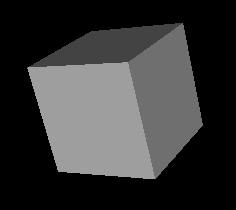
\includegraphics[]{./cube.png}
\caption{\label{cube} \textit{Le Cube}.}
\end{center}
\end{figure}


\begin{tabular}[t]{|c|c|c|c||c|c|c|}
\hline
 Mod�le             & Points & Ar�tes & Faces & Triangles & Quads & Autres \\
\hline
 Cube               & 8      & 12     & 6     & 0         & 6     & 0 \\
\hline
\hline
                    & \multicolumn{2}{|c|}{Test 1} & \multicolumn{2}{|c|}{Test 2} & \multicolumn{2}{|c|}{Test 3} \\
\hline
 Nb. V�rifications  &  \multicolumn{2}{|c|}{RESULTAT} & \multicolumn{2}{|c|}{RESULTAT}  &  \multicolumn{2}{|c|}{RESULTAT} \\     
\hline
\hline
 \begin{tabular}[t]{c|c}
  Mantilla & 
     \begin{tabular}[t]{c} 
			 $\varepsilon = 1.0$ \\
			 $\varepsilon = 0.0$ \\
			 $\varepsilon = 0.5$ \\
			 $\varepsilon = 0.1$ \\
			 $\varepsilon = 0.001$ \\
			 $\varepsilon = 10^{-6}$ \\
			 $\varepsilon = 10^{-14}$ \\
		 \end{tabular}\\
 \end{tabular} & 
   \multicolumn{2}{|c|}{
		\begin{tabular}[t]{c}
			RESULTAT \\ 
			RESULTAT \\
			RESULTAT \\
			RESULTAT \\
			RESULTAT \\
			RESULTAT \\
			RESULTAT 
	 \end{tabular} } & 
	 \multicolumn{2}{|c|}{
		\begin{tabular}[t]{c}
			RESULTAT \\ 
			RESULTAT \\
			RESULTAT \\
			RESULTAT \\
			RESULTAT \\
			RESULTAT \\
			RESULTAT 
		\end{tabular}	 
	 } & 	
	 \multicolumn{2}{|c|}{
		 	\begin{tabular}[t]{c}
			RESULTAT \\ 
			RESULTAT \\
			RESULTAT \\
			RESULTAT \\
			RESULTAT \\
			RESULTAT \\
			RESULTAT 
	 \end{tabular}
	 }\\
\hline
\hline
CORE &   
\multicolumn{2}{|c|}{RESULTAT} &  
\multicolumn{2}{|c|}{RESULTAT} & 
\multicolumn{2}{|c|}{RESULTAT} \\
\hline
\end{tabular}


\begin{figure}[h!]
\begin{center}
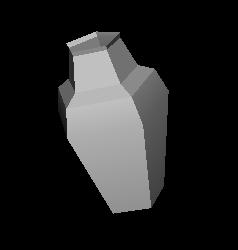
\includegraphics[]{./vase.png}
\caption{\label{vase} 
\textit{Vase}.}
\end{center}
\end{figure}

\begin{tabular}[t]{|c|c|c|c||c|c|c|}
\hline
 Mod�le             & Points & Ar�tes & Faces & Triangles & Quads & Autres \\
\hline
 Cube               & 8      & 12     & 6     & 0         & 6     & 0 \\
\hline
\hline
                    & \multicolumn{2}{|c|}{Test 1} & \multicolumn{2}{|c|}{Test 2} & \multicolumn{2}{|c|}{Test 3} \\
\hline
 Nb. V�rifications  &  \multicolumn{2}{|c|}{RESULTAT} & \multicolumn{2}{|c|}{RESULTAT}  &  \multicolumn{2}{|c|}{RESULTAT} \\     
\hline
\hline
 \begin{tabular}[t]{c|c}
  Mantilla & 
     \begin{tabular}[t]{c} 
			 $\varepsilon = 1.0$ \\
			 $\varepsilon = 0.0$ \\
			 $\varepsilon = 0.5$ \\
			 $\varepsilon = 0.1$ \\
			 $\varepsilon = 0.001$ \\
			 $\varepsilon = 10^{-6}$ \\
			 $\varepsilon = 10^{-14}$ \\
		 \end{tabular}\\
 \end{tabular} & 
   \multicolumn{2}{|c|}{
		\begin{tabular}[t]{c}
			RESULTAT \\ 
			RESULTAT \\
			RESULTAT \\
			RESULTAT \\
			RESULTAT \\
			RESULTAT \\
			RESULTAT 
	 \end{tabular} } & 
	 \multicolumn{2}{|c|}{
		\begin{tabular}[t]{c}
			RESULTAT \\ 
			RESULTAT \\
			RESULTAT \\
			RESULTAT \\
			RESULTAT \\
			RESULTAT \\
			RESULTAT 
		\end{tabular}	 
	 } & 	
	 \multicolumn{2}{|c|}{
		 	\begin{tabular}[t]{c}
			RESULTAT \\ 
			RESULTAT \\
			RESULTAT \\
			RESULTAT \\
			RESULTAT \\
			RESULTAT \\
			RESULTAT 
	 \end{tabular}
	 }\\
\hline
\hline
CORE &   
\multicolumn{2}{|c|}{RESULTAT} &  
\multicolumn{2}{|c|}{RESULTAT} & 
\multicolumn{2}{|c|}{RESULTAT} \\
\hline
\end{tabular}

\begin{figure}[h!]
\begin{center}
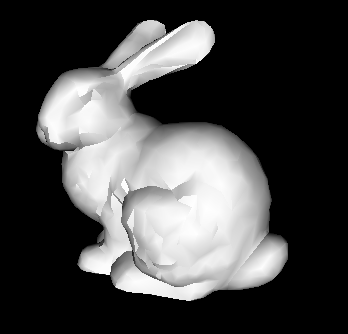
\includegraphics[]{./bunny.png}
\caption{\label{bunny} 
\textit{Le Lapin. Mod�le VRML simplifi� du	mod�le original de Standford}.}
\end{center}
\end{figure}

\begin{figure}[h!]
\begin{center}
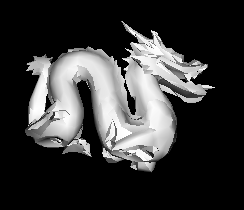
\includegraphics[]{./dragon.png}
\caption{\label{dragon} 
\textit{Le Dragon. Mod�le VRML simplifi� du	mod�le original de Standford}.}
\end{center}
\end{figure}

\begin{figure}[h!]
\begin{center}
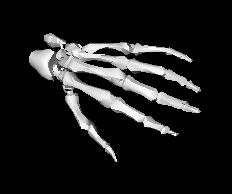
\includegraphics[]{./hand.png}
\caption{\label{hand} 
\textit{Main. Mod�le VRML simplifi� du	mod�le original de Standford}.}
\end{center}
\end{figure}


\begin{figure}[h!]
\begin{center}
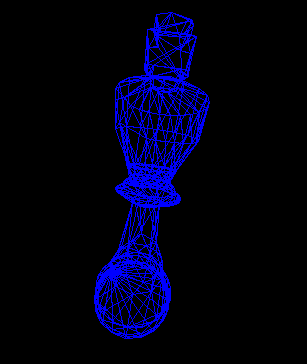
\includegraphics[]{./chess1.png}
\caption{\label{chess1} 
\textit{Pi�ce d'�chec}.}
\end{center}
\end{figure}

\begin{figure}[h!]
\begin{center}
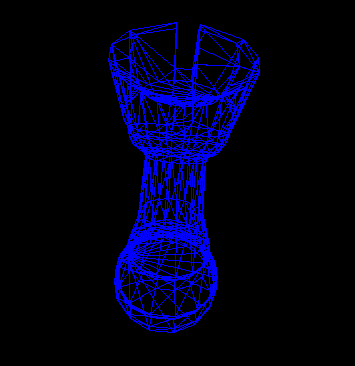
\includegraphics[]{./chess2.png}
\caption{\label{chess2} 
\textit{Pi�ce d'�chec}.}
\end{center}
\end{figure}

\begin{figure}[h!]
\begin{center}
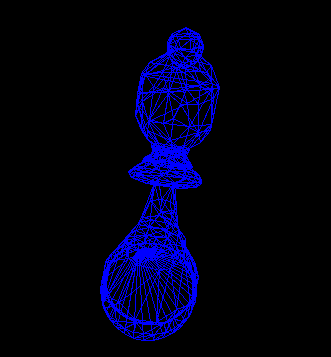
\includegraphics[]{./chess3.png}
\caption{\label{chess3} 
\textit{Pi�ce d'�chec}.}
\end{center}
\end{figure}


\onecolumn

\section{Discussion et Conclusion}

\end{document}
